
%%%%%%%%%%%%%%%%%%%%%%%%%%%%%%%%%%%%%%%%%%%%
\section{The Future Engineering }

{
\paper{\textbf{Xochicale 2020} in Conf. of Reproducibility, Replicability and Trust in Science \faGithub github.com/mxochicale/rrts2020}
\begin{frame}{Introduction}
      \begin{figure}
        \centering
        %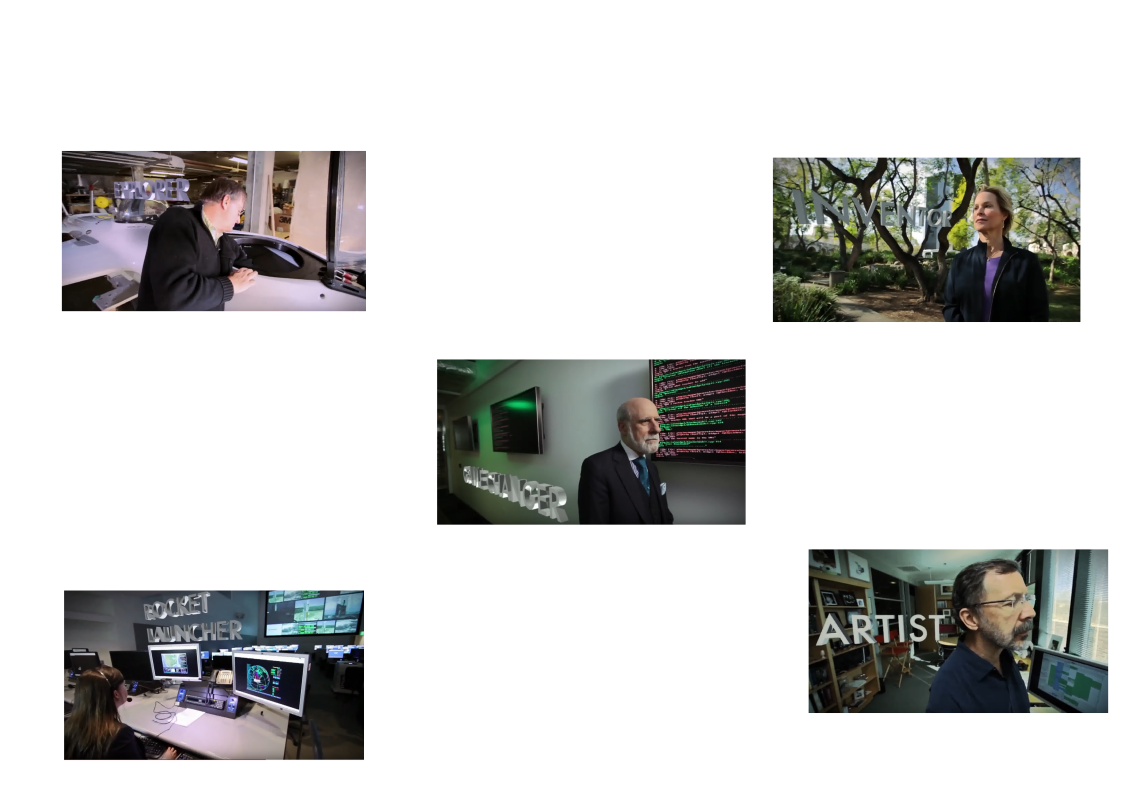
\includegraphics[width=\linewidth]{./figs/eng-of-the-future/versions/drawing.png}
        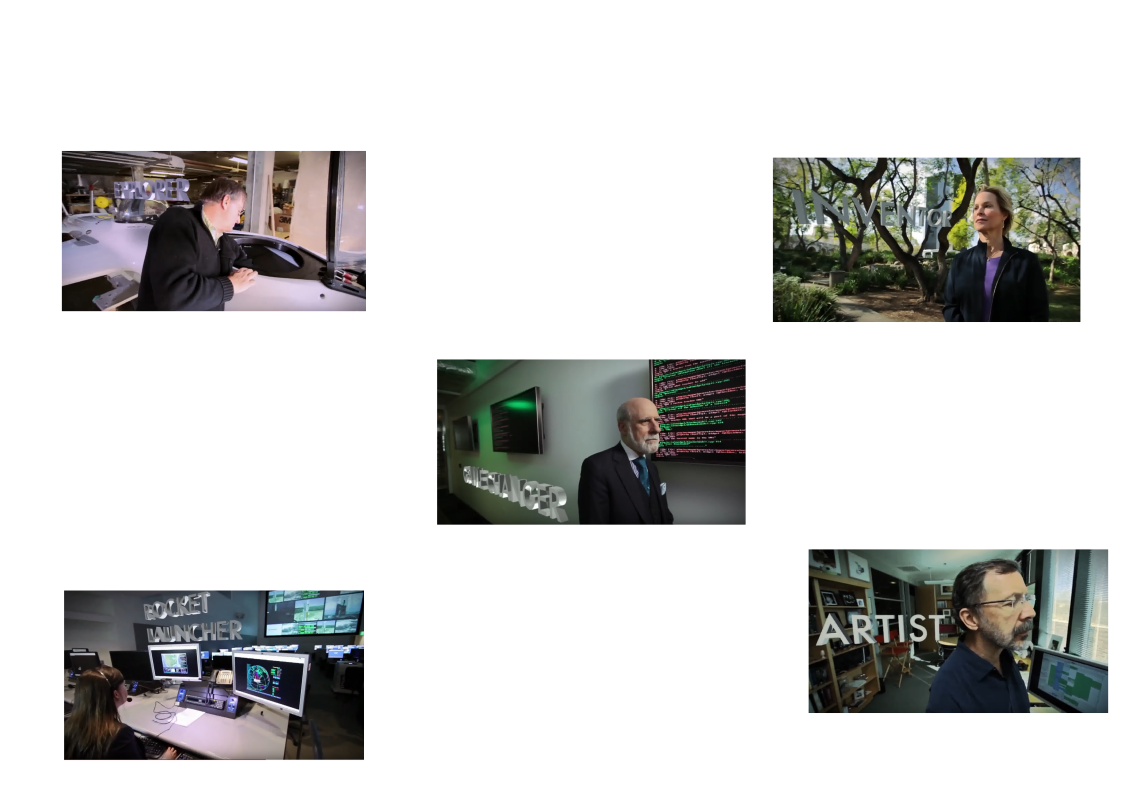
\includegraphics[scale=0.2]{./figs/eng-of-the-future/versions/drawing.png}
        \caption{Compile \LaTeX~Project in VSCode}
      \end{figure}

\end{frame}
}


\begin{frame}{Introduction}
  \begin{itemize}
    \item \alert{\LaTeX{}} is a document preparation system and document markup language.
    \item It can be used to typeset articles, books, slides, posters, even graphics.
    \item \textbf{\textcolor{Green}{Pros}:}
          \begin{itemize}
            \item It separates presentation/format from contents.
            \item Since the source codes are plaintext, it works well with version control system such as git.
            \item Highly customizable through various of packages.
          \end{itemize}
    \item \textbf{\textcolor{Red}{Cons}:}
          \begin{itemize}
            \item There is no graphic interface to support WYSIWYG style editing.
            \item Not suitable to produce unstructured documents.
          \end{itemize}
  \end{itemize}
\end{frame}


